\icode{E-EME-SI-L2-261121-003}
如图所示，真空中\(A\)、\(B\)两点分别固定两个相同的带电金属小球（均可视为点电荷），所带电荷量分别为\( + Q\)和\( - 5Q \)，在\(A\)、\(B\)的延长线上的\(C\)点处固定一电荷量为\(q\)的试探电荷，试探电荷受到的电场力大小为\(F_1\)，已知\(AB = BC\)。若将两带电金属小球接触后再放回\(A\)、\(B\)两处时，试探电荷受到的电场力大小为\(F_2\)，则\(\frac{F_1}{F_2}\)为\paren[]
	
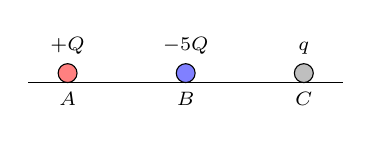
\begin{tikzpicture}[>=stealth,font=\scriptsize]
	\foreach \c/\cr/\n/\a in {(-1.5,0)/red/+Q/A,(0,0)/blue/-5Q/B,(1.5,0)/gray/q/C}{
		\draw \c--++(0,-.12)node[below]{\(\a\)};
		\draw \c--++(0,.12)node[above]{\(\n\)};
		\draw[fill=\cr!50] \c circle(.12);}
	\draw (-2,-.12)--(2,-.12);
\end{tikzpicture}
\begin{choices}
	\item \(\frac{21}{20}\)
	\item \(\frac{21}{16}\)
	\item \(\frac{19}{10}\)
	\item \(\frac{19}{16}\)
\end{choices}
\begin{answer}
	C\qquad 提示：
\end{answer}